%!TEX root = ../Implementation.tex

\chapter{Working Methodology}
\label{sec:methodology}

This chapter provides an overview of the methodology applied during the implementation of the Codex project. In particular, it discusses the comparison between the originally planned schedule and the actual project timeline. Furthermore, the technical infrastructure used during development, as well as the coordination and communication within the team, are described.

\section{Schedule}
\label{subsec:schedule}

Figure \ref{fig:gantt-planned} shows a Gantt-Chart of the planned implementation schedule that was created in the beginning of the phase. 
 
\begin{figure}[H]
    \centering
    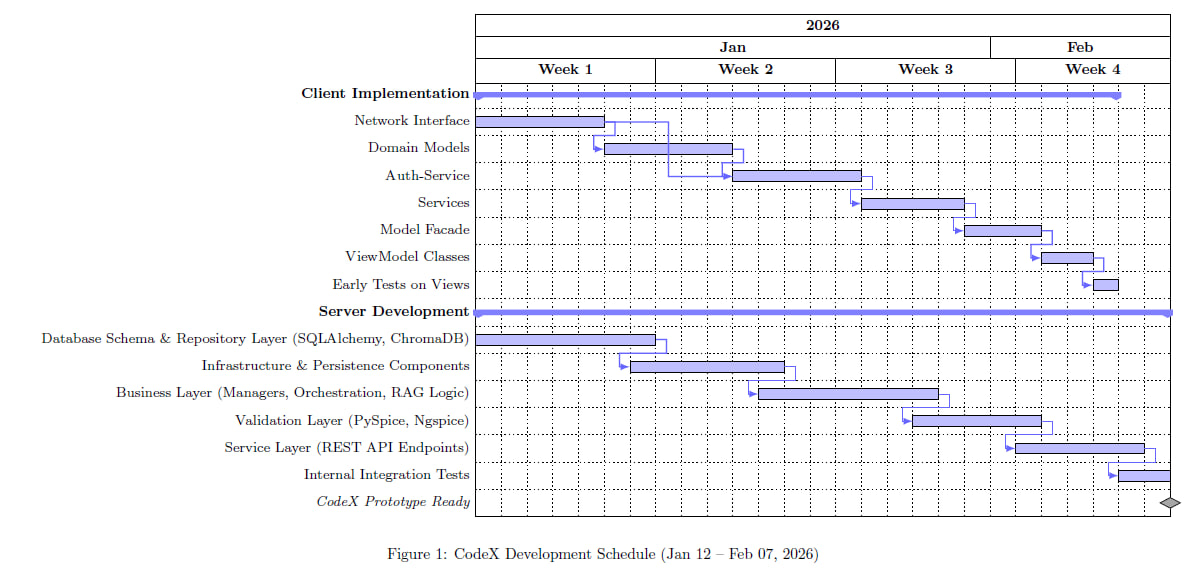
\includegraphics[width=1.1\textwidth]{figures/gannt_planned.jpg}
    \caption{Planned Project Timeline}
    \label{fig:gantt-planned}
\end{figure}

The actual implementation strayed far from this planned approach. While the general structure was followed, the linear approach could not be adhered to.
Instead, some components were developed simultaneously to get immediate feedback and to allow manual testing before a component was fully finished. \\

The changes that were made to the architecture also affected the schedule. After identifying a problem in the architecture, the already implemented parts needed to be re-adjusted to the changes. This happened several times in both the server and client.

\section{Empirical Schedule}
The empirically track the progress made on the code-base, we used data provided by the git-history of both projects. See Figure \ref{fig:empirical-client-loc} and \ref{fig:empirical-server-loc} for an overview of the Lines of Code.

\begin{figure}
    \centering
    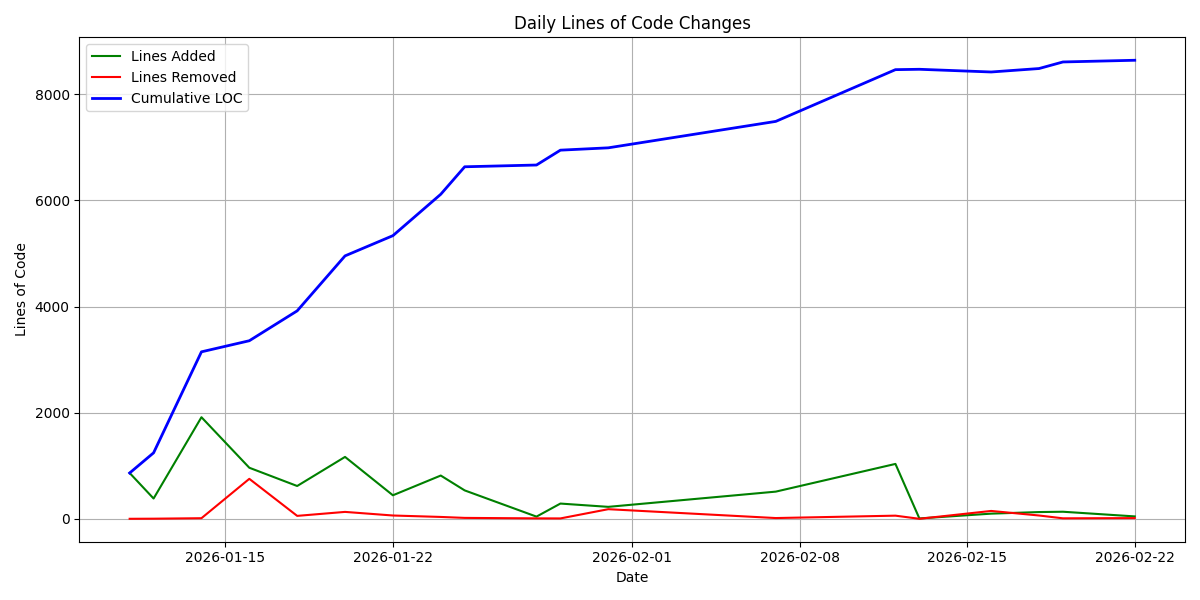
\includegraphics[width=0.8\textwidth]{figures/client_loc.png}
    \caption{Empirical Client Lines of Code}
    \label{fig:empirical-client-loc}
\end{figure}

\begin{figure}
    \centering
    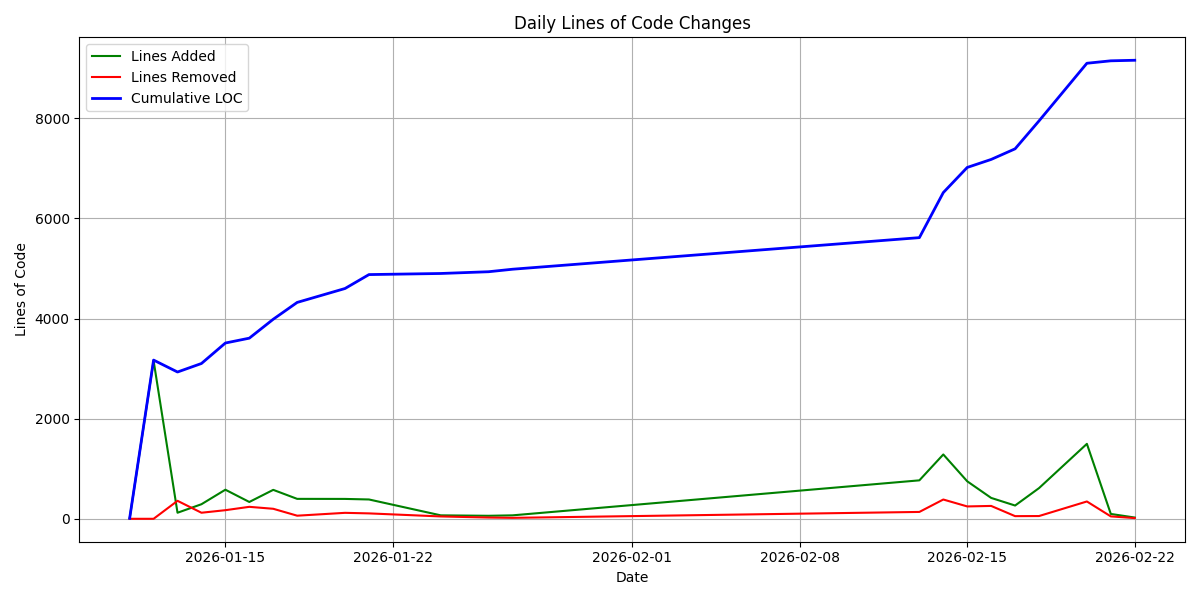
\includegraphics[width=0.8\textwidth]{figures/server_loc.png}
    \caption{Empirical Server Lines of Code}
    \label{fig:empirical-server-loc}
\end{figure}

\section{Analysis of Difficulties}
\label{subsec:analysis-delays}

The learning curve associated with the chosen technologies, especially in the context of asynchronous request handling and interactive client-side visualization, was steeper than originally estimated. Additionally, the implementation of robust error handling and validation mechanisms required more effort than planned.

Unforeseen issues, such as unexpected bugs and integration problems, as well as human factors, also had an effect on the implementation. Over the course of the project, however, the team benefited from a noticeable learning effect. As a result, later development tasks could be completed more efficiently despite the initial delays.

In some cases, delays were mitigated by parallelizing development activities. For example, client-side visualization components and server-side processing logic were partially developed in parallel once stable interfaces had been defined. Nevertheless, certain trade-offs were necessary. In particular, some optional features and a more extensive test coverage had to be deprioritized in order to meet the overall project deadline.

\subsection{Internal Communication}
\label{subsec:internal-communication}

Effective communication was a key factor in the successful implementation of the Codex project. The development team relied on a combination of digital tools and regular in-person meetings to stay coordinated. WhatsApp was used for day-to-day communication, enabling quick questions, status updates, and immediate coordination, while Discord facilitated more technical discussions, including design decisions, problem-solving, and real-time collaboration, particularly for remote team members.

Regular on-site meetings complemented the digital communication by allowing face-to-face discussions of project progress, upcoming tasks, and complex issues. This blended approach ensured that team members remained aligned and informed, with clear documentation of decisions, well-defined responsibilities, and prompt resolution of misunderstandings. Overall, this structured communication strategy contributed significantly to efficient coordination and helped the team navigate technical challenges effectively.

\section{Technical Development Environment and Infrastructure}
\label{subsec:technical-environment}

This section describes the technical development environment and infrastructure used during the implementation of the Codex project. It covers the development environments employed by the team, the tools used for implementation, as well as the version control strategy and its evolution over the course of the project.

\subsection{Integrated Development Environment}
\label{subsubsec:ide}

Within the development team, no single, unified Integrated Development Environment (IDE) was enforced.
Given the fact that IDE's are only supportive tools, every member used their own individual approach.
Namely, the following IDE's were used:

\begin{itemize}
    \item Jetbrains PyCharm
    \item Jetbrains Intellij IDEA Ultimate
    \item Jetbrains WebStorm
    \item Visual Studio Code
\end{itemize}

\subsection{Development Tools}
\label{subsubsec:dev-tools}

For backend development, no dedicated or standardized development tools were enforced beyond the selected IDEs. The project did not rely on a centralized build system, automated formatting tools, or static code analysis frameworks.

Instead, development was carried out using the built-in functionality of the respective development environments. Code structure, formatting, and quality were maintained manually by the team members according to agreed conventions.

Furthermore, no automated pipelines or integrated quality assurance tools were used during development. Dependency management and configuration were handled directly by the respectively used framework.

\subsection{Version Control}
\label{subsubsec:version-control}

Git was used as the version control system for the project. Each team member worked with an individual local repository, while a shared remote repository (for each, server and client) hosted on GitHub was used to coordinate development and integrate contributions.

From the beginning of the project, development was organized using a structured branching strategy. Separate branches were created for individual layers of the application as well as for smaller, clearly defined tasks. In most cases, a single team member was responsible for implementing and maintaining a branch.

When necessary, collaboration on a branch took place without complications. The scope of tasks was clearly defined, which prevented overlapping changes and minimized the risk of conflicts. As a result, the team did not encounter significant merge conflicts during development.

Pull requests were used to integrate completed work into the main branch. Since responsibilities and task boundaries were well coordinated, merges were performed in a controlled and orderly manner. No fast-forward merge strategy was specifically enforced, as the existing workflow already ensured a clear and understandable project history.

Overall, the consistent branching structure and clear task allocation enabled smooth collaboration throughout the entire implementation phase.